\UseRawInputEncoding

%%%%%%%%%%%%%%%%%%%%%%%%%%%%%%%%%%%%%%%%%%%%%%%%%%%%%%%%%%%%%%%%%%%%%%%%%%%%%%%%
%% SETTINGS
%%%%%%%%%%%%%%%%%%%%%%%%%%%%%%%%%%%%%%%%%%%%%%%%%%%%%%%%%%%%%%%%%%%%%%%%%%%%%%%%
%% Columns
\documentclass[final,3p,times,twocolumn]{elsarticle}
%% Use the options 1p,twocolumn; 3p; 3p,twocolumn; 5p; or 5p,twocolumn
%% for a journal layout:
%% \documentclass[final,1p,times]{elsarticle}
%% \documentclass[final,1p,times,twocolumn]{elsarticle}
%% \documentclass[final,3p,times]{elsarticle}
%% \documentclass[final,3p,times,twocolumn]{elsarticle}
%% \documentclass[final,5p,times]{elsarticle}
%% \documentclass[final,5p,times,twocolumn]{elsarticle}
%% \documentclass[preprint,review,12pt]{elsarticle}

%% Image width
\newlength{\imagewidth}
\newlength{\imagescale}
%% preamble
\usepackage[english]{babel}
\usepackage[table]{xcolor} % For coloring tables
\usepackage{booktabs} % For professional quality tables
\usepackage{colortbl} % For coloring cells in tables
\usepackage{amsmath, amssymb} % For mathematical symbols and environments
\usepackage{amsthm} % For theorem-like environments
\usepackage{lipsum} % just for sample text
\usepackage{natbib}
\usepackage{graphicx}
\usepackage{indentfirst}
\usepackage{bashful}
\usepackage[margin=10pt,font=small,labelfont=bf,labelsep=endash]{caption}
\usepackage{graphicx}
\usepackage{calc}
\usepackage[T1]{fontenc} % [REVISED]
\usepackage[utf8]{inputenc} % [REVISED]
\usepackage{hyperref}
\usepackage{accsupp}
%% Line numbers
\linespread{1.1}
% \linenumbers
% Tables
\usepackage[pass]{geometry}
\usepackage{pdflscape}
\usepackage{csvsimple}
\usepackage{xltabular}
\usepackage{booktabs}
\usepackage{siunitx}
\usepackage{makecell}
\sisetup{round-mode=figures,round-precision=3}
\renewcommand\theadfont{\bfseries}
\renewcommand\theadalign{c}
\newcolumntype{C}[1]{>{\centering\arraybackslash}m{#1}}
\renewcommand{\arraystretch}{1.5}
\definecolor{lightgray}{gray}{0.95}

%% Diff
\usepackage{xcolor}
% Define commands for highlighting
% diff
\usepackage[most]{tcolorbox} % for boxes with transparency
% Define colors with transparency (opacity value)
\definecolor{GreenBG}{rgb}{0,1,0}
\definecolor{RedBG}{rgb}{1,0,0}
% Define tcolorbox environments for highlighting
\newtcbox{\greenhighlight}[1][]{%
  on line,
  colframe=GreenBG,
  colback=GreenBG!50!white, % 50% transparent green
  boxrule=0pt,
  arc=0pt,
  boxsep=0pt,
  left=1pt,
  right=1pt,
  top=2pt,
  bottom=2pt,
  tcbox raise base
}
\newtcbox{\redhighlight}[1][]{%
  on line,
  colframe=RedBG,
  colback=RedBG!50!white, % 50% transparent red
  boxrule=0pt,
  arc=0pt,
  boxsep=0pt,
  left=1pt,
  right=1pt,
  top=2pt,
  bottom=2pt,
  tcbox raise base
}
\newcommand{\REDSTARTS}{\color{red}}
\newcommand{\REDENDS}{\color{black}}
\newcommand{\GREENSTARTS}{\color{green}}
\newcommand{\GREENENDS}{\color{black}}

% New command to read word counts
\newread\wordcount
\newcommand\readwordcount[1]{%
  \openin\wordcount=#1
  \read\wordcount to \thewordcount
  \closein\wordcount
  \thewordcount
}

%%%%%%%%%%%%%%%%%%%%%%%%%%%%%%%%%%%%%%%%%%%%%%%%%%%%%%%%%%%%%%%%%%%%%%%%%%%%%%%%
%% JOURNAL NAME
%%%%%%%%%%%%%%%%%%%%%%%%%%%%%%%%%%%%%%%%%%%%%%%%%%%%%%%%%%%%%%%%%%%%%%%%%%%%%%%%
\journal{Heliyon}
%%%%%%%%%%%%%%%%%%%%%%%%%%%%%%%%%%%%%%%%%%%%%%%%%%%%%%%%%%%%%%%%%%%%%%%%%%%%%%%%
%% DOCUMENT STARTS
%%%%%%%%%%%%%%%%%%%%%%%%%%%%%%%%%%%%%%%%%%%%%%%%%%%%%%%%%%%%%%%%%%%%%%%%%%%%%%%%
\begin{document}

%%%%%%%%%%%%%%%%%%%%%%%%%%%%%%%%%%%%%%%%%%%%%%%%%%%%%%%%%%%%%%%%%%%%%%%%%%%%%%%%
%% Frontmatter
%%%%%%%%%%%%%%%%%%%%%%%%%%%%%%%%%%%%%%%%%%%%%%%%%%%%%%%%%%%%%%%%%%%%%%%%%%%%%%%%
\begin{frontmatter}
\begin{highlights}
\pdfbookmark[1]{Highlights}{highlights}

\item Neural trajectories in the hippocampus exhibited greater variability during a working memory (WM) task compared to those in the entorhinal cortex and amygdala regions.

\item The distance of neural trajectories between encoding and retrieval states in the hippocampus was memory-load dependent during a WM task.


\item Hippocampal neural trajectories fluctuated between the encoding and retrieval states in a task-dependent manner during both baseline and sharp-wave ripple (SWR) periods.

\item Hippocampal neural trajectories shifted from encoding to retrieval states during SWR period.

\end{highlights}\title{
Hippocampal Neural Fluctuations Between Memory Encoding and Retrieval States During a Working Memory Task in Humans
}\author[1]{Yusuke Watanabe\corref{cor1}}
\author[2,3,4]{Yuji Ikegaya}
\author[1,5]{Takufumi Yanagisawa}

\address[1]{Institute for Advanced Cocreation studies, Osaka University, 2-2 Yamadaoka, Suita, 565-0871, Osaka, Japan}
\address[2]{Graduate School of Pharmaceutical Sciences, The University of Tokyo, 7-3-1 Hongo, Tokyo, 113-0033, Japan}
\address[3]{Institute for AI and Beyond, The University of Tokyo, 7-3-1 Hongo, Tokyo, 113-0033, Japan}
\address[4]{Center for Information and Neural Networks, National Institute of Information and Communications Technology, 1-4 Yamadaoka, Suita City, 565-0871, Osaka, Japan}
\address[5]{Department of Neurosurgery, Osaka University Graduate School of Medicine, 2-2 Yamadaoka, Osaka, 565-0871, Japan}

\cortext[cor1]{Corresponding author. Tel: +81-6-6879-3652 Email: ywatanabe@alumni.u-tokyo.ac.jp}

%%Graphical abstract
%\pdfbookmark[1]{Graphical Abstract}{graphicalabstract}        
%\begin{graphicalabstract}
%\includegraphics{grabs}
%\end{graphicalabstract}
\begin{abstract}
\pdfbookmark[1]{Abstract}{abstract}
Working memory (WM) is vital for many cognitive functions, although the neural mechanisms underlying its operation are not yet fully understood. Although the hippocampus and associated sharp-wave ripples (SWRs) --- brief, synchronized oscillations within it --- have been explored owing to their role in memory consolidation and retrieval, a comprehensive understanding of their involvement in WM tasks is pending further investigation. This study reveals that a WM task introduces unique dynamics into the multi-unit activity patterns of the hippocampus, primarily during SWR episodes. We analyzed intracranial electroencephalography data collected from the medial temporal lobe (MTL) of nine epilepsy patients performing an eight-second Sternberg task. Using Gaussian-process factor analysis, we extracted low-dimensional neural representations or neural trajectories (NT) within MTL regions throughout the Sternberg WM task. The analysis demonstrated substantial differences in hippocampal NT compared to that in the entorhinal cortex and the amygdala. Additionally, the NT distance between the encoding and retrieval phases was dependent on the memory load. Notably, hippocampal NT distinguished encoding and retrieval states during the retrieval phase in a task-dependent manner. These differences transitioned from encoding to retrieval states in the presence of SWR episodes. These results emphasize the importance of the hippocampus in WM tasks and propose a new hypothesis: the hippocampus transitions its functional state from encoding to retrieval during SWRs in WM tasks.
\end{abstract}% \pdfbookmark[1]{Keywords}{keywords}                
\begin{keyword}
working memory \sep memory load \sep hippocampus \sep sharp-wave ripples \sep humans
\end{keyword}
\end{frontmatter}

%%%%%%%%%%%%%%%%%%%%%%%%%%%%%%%%%%%%%%%%%%%%%%%%%%%%%%%%%%%%%%%%%%%%%%%%%%%%%%%%
%% Counters
%%%%%%%%%%%%%%%%%%%%%%%%%%%%%%%%%%%%%%%%%%%%%%%%%%%%%%%%%%%%%%%%%%%%%%%%%%%%%%%%
\begin{wordcount*}
\readwordcount{./src/.figure_count.txt} figures, \readwordcount{./src/.table_count.txt} tables, \readwordcount{./src/.abstract_count.txt} words for abstract, and \readwordcount{./src/.imrd_count.txt} words for main text
\end{wordcount*}
%%%%%%%%%%%%%%%%%%%%%%%%%%%%%%%%%%%%%%%%%%%%%%%%%%%%%%%%%%%%%%%%%%%%%%%%%%%%%%%%
%% IMRaD
%%%%%%%%%%%%%%%%%%%%%%%%%%%%%%%%%%%%%%%%%%%%%%%%%%%%%%%%%%%%%%%%%%%%%%%%%%%%%%%%

%%%%%%%%%%%%%%%%%%%%%%%%%%%%%%%%%%%%%%%%%%%%%%%%%%%%%%%%%%%%%%%%%%%%%%%%%%%%%%%%
%% INTRODUCTION
%%%%%%%%%%%%%%%%%%%%%%%%%%%%%%%%%%%%%%%%%%%%%%%%%%%%%%%%%%%%%%%%%%%%%%%%%%%%%%%%
\section{Introduction}
Working memory (WM) plays an essential role in everyday activities, yet comprehensive understanding of its neural mechanism, including the hippocampus's involvement in WM processing, remains elusive. The hippocampus, a central region for memory, is the focus of continuous research \cite{scoville_loss_1957} \cite{squire_legacy_2009}  \cite{boran_persistent_2019} \cite{kaminski_persistently_2017} \cite{kornblith_persistent_2017} \cite{faraut_dataset_2018} \cite{borders_hippocampus_2022} \cite{li_functional_2023} \cite{dimakopoulos_information_2022}. Gaining insight into the role of the hippocampus in working memory is key to enhancing our understanding of cognitive processes and could potentially improve cognitive capabilities.
\\
\indent
Current evidence suggests that sharp-wave ripples (SWRs), a form of transient, synchronized oscillation, is linked with several cognitive functions. These functions include memory replay \cite{wilson_reactivation_1994} \cite{nadasdy_replay_1999} \cite{lee_memory_2002} \cite{diba_forward_2007} \cite{davidson_hippocampal_2009}, memory consolidation \cite{girardeau_selective_2009} \cite{ego-stengel_disruption_2010} \cite{fernandez-ruiz_long-duration_2019} \cite{kim_corticalhippocampal_2022}, memory recall \cite{wu_hippocampal_2017} \cite{norman_hippocampal_2019} \cite{norman_hippocampal_2021}, and neural plasticity \cite{behrens_induction_2005} \cite{norimoto_hippocampal_2018}. These ties suggest that SWR serve as a fundamental computational mechanism of hippocampal processing, contributing to the performance of working memory.
\\
\indent
Recent studies show that low-dimensional representations in hippocampal neurons can account for WM task performance. In particular, the firing patterns of place cells \cite{okeefe_hippocampus_1971} \cite{okeefe_place_1976} \cite{ekstrom_cellular_2003} \cite{kjelstrup_finite_2008} \cite{harvey_intracellular_2009}, found in the hippocampus, were noted within dynamic, nonlinear three-dimensional hyperbolic spaces in rats \cite{zhang_hippocampal_2022}. Also, grid cells in the entorhinal cortex (EC)—the key conduit to the hippocampus \cite{naber_reciprocal_2001} \cite{van_strien_anatomy_2009} \cite{strange_functional_2014}—demonstrated toroidal geometry during exploration in rats \cite{gardner_toroidal_2022}.
\\
\indent
However, these studies primarily concentrate on spatial navigation in rodents and consequently, feature limitations. For instance, the temporal resolution of navigation tasks is insufficient because the timing of memory acquisition and recall has not been clearly defined. As a result, there are few studies examining the influence of SWRs on WM performance \cite{jadhav_awake_2012}. Furthermore, the existence of noise in signals recorded during rodent movement complicates the detection of SWRs \cite{Watanabe_2021}. Hence, human research is needed to elucidate the relationship between SWRs and WM tasks.
\\
\indent
Taking these factors into account, this study explores the hypothesis that during SWR periods, hippocampal neurons exhibit distinct neural trajectories (NTs) in low-dimensional space in response to WM tasks in humans. To substantiate this hypothesis, we used a dataset of patients performing an eight-second Sternberg task (one second for fixation, two seconds for encoding, three seconds for maintenance, and two seconds for retrieval) with high temporal resolution. For these patients, intracranial electroencephalography (iEEG) signals within the medial temporal lobe (MTL) were recorded \cite{boran_dataset_2020}. To investigate low-dimensional NTs, we employed Gaussian-process factor analysis (GPFA), a proven method for analyzing neural population dynamics \cite{yu_gaussian-process_2009}.
\label{sec:introduction}
%%%%%%%%%%%%%%%%%%%%%%%%%%%%%%%%%%%%%%%%%%%%%%%%%%%%%%%%%%%%%%%%%%%%%%%%%%%%%%%%
%% METHODS
%%%%%%%%%%%%%%%%%%%%%%%%%%%%%%%%%%%%%%%%%%%%%%%%%%%%%%%%%%%%%%%%%%%%%%%%%%%%%%%%
\section{Methods}
\subsection{Dataset}
The data for this study were obtained from a publicly available dataset involving nine patients with epilepsy performing a modified Sternberg task \cite{boran_dataset_2020}. This task encompasses four stages: fixation (1s), encoding (2s), maintenance (3s), and retrieval (2s). During the encoding phase, a set of four, six, or eight letters were presented to the participants. Subsequently, they were tasked with assessing whether a probe letter displayed during the retrieval phase was previously shown (indicating a correct response for the Match IN task) or not (indicating a correct response for the Mismatch OUT task). Intracranial electroencephalography (iEEG) signals were recorded at a 32 kHz sampling rate within a 0.5--5,000 Hz frequency range, with depth electrodes placed in medial temporal lobe (MTL) regions including the anterior head and posterior body of the left and right hippocampus (AHL, AHR, PHL, and PHR), the entorhinal cortex (ECL and ECR), and the amygdala (AL and AR), as shown in Figure~\ref{fig:01}A and Table~\ref{tab:01}. The iEEG signals were then downsampled to 2 kHz. Correlations between variables such as set size and accuracy rate were explored (Figure~\ref{fig:s01}S1). Multiunit spike timings were determined via a spike sorting algorithm \cite{niediek_reliable_2016} using the Combinato package (\url{https://github.com/jniediek/combinato})(Figure~\ref{fig:01}C).

\subsection{Calculation of NT using GPFA}
Neural trajectories (NTs), also referred to as 'factors', in the hippocampus, EC, and amygdala were identified using Gaussian-Process Factor Analysis (GPFA) \cite{yu_gaussian-process_2009} applied to multi-unit activity data for each session, using the Elephant package (\url{https://elephant.readthedocs.io/en/latest/reference/gpfa.html}). The bin size was set to 50 ms with no overlaps. Each factor was Z-normalized across all sessions, and the Euclidean distance from the origin (O) was computed.
\\
\indent
For each NT in respective regions like AHL, geometric medians ($\mathrm{g_{F}}$ for fixation, $\mathrm{g_{E}}$ for encoding, $\mathrm{g_{M}}$ for maintenance, and $\mathrm{g_{R}}$ for retrieval phase) were calculated by determining the NT's median coordinates during the four phases. An optimal GPFA dimensionality was identified as three using the elbow method drawn from investigating the log-likelihood values via a three-fold cross-validation approach (Figure~\ref{fig:02}B).

\subsection{Identifying SWR candidates from hippocampal regions}
Potential sharp wave-ripple (SWR) events within the hippocampus were identified using a widely accepted method \cite{liu_consensus_2022}. Local field potential (LFP) signals from a region of interest (ROI), such as AHL, were re-referenced by deducting the averaged signal from locations outside the ROI (including AHR, PHL, PHR, ECL, ECR, AL, and AR). The re-referenced LFP signals were then filtered using a ripple-band filter (80--140 Hz) to identify SWR candidates, denoted as $\textrm{SWR}^+$ candidates. SWR detection used a published tool (\url{https://github.com/Eden-Kramer-Lab/ripple_detection}) \cite{kay_hippocampal_2016}, with the bandpass range adjusted to 80--140 Hz for humans \cite{norman_hippocampal_2019, norman_hippocampal_2021}, unlike the initial 150--250 Hz range typically applied to rodents.
\\
\indent
Control events for $\textrm{SWR}^+$ candidates, labeled as $\textrm{SWR}^-$ candidates, were discovered by randomly shuffling the timestamps of $\textrm{SWR}^+$ candidates across all trials and subjects. The resulting $\textrm{SWR}^+/\textrm{SWR}^-$ candidates were then visually inspected.

\subsection{Defining SWRs from potential hippocampal CA1 regions}
Candidates for $\textrm{SWR}^+/\textrm{SWR}^-$ events in the hippocampus' putative CA1 regions were distinguished. Pyramidal neurons in these regions, referred to as cornu ammonis 1 (CA1), were initially defined as follows: $\textrm{SWR}^+/\textrm{SWR}^-$ candidates were projected into a two-dimensional space based on overlapping spike counts per unit using a supervised method, UMAP (Uniform Manifold Approximation and Projection) \cite{mcinnes_umap_2018}. Clustering validation was performed by calculating the silhouette score \cite{rousseeuw_silhouettes_1987} from clustered samples. Regions in the hippocampus, with scores above 0.6 on average across sessions (75th percentile), were classified as putative CA1 regions, resulting in the identification of five electrode positions from five patients.
\\
\indent
$\textrm{SWR}^+/\textrm{SWR}^-$ candidates in these predefined CA1 regions were marked as $\textrm{SWR}^+/\textrm{SWR}^-$, consequently losing their candidate status. The duration and ripple band peak amplitude of SWRs were found to follow log-normal distributions. Each SWR timeframe was partitioned relative to the time from the SWR center into pre- (at $-800$ ms to $-300$ ms from the SWR center), mid- (at $-250$ to $+250$ ms), and post-SWR (at $+300$ to $+800$ ms) periods.

\subsection{Statistical Evaluation}
Both the Brunner--Munzel test and the Kruskal-Wallis test were performed using the SciPy package in Python \cite{virtanen_scipy_2020}. Correlational analysis was conducted by determining the rank of the observed correlation coefficient within its associated set-size-shuffled surrogate using a custom Python script. The bootstrap test was implemented with an in-house Python script.
\label{sec:methods}
%%%%%%%%%%%%%%%%%%%%%%%%%%%%%%%%%%%%%%%%%%%%%%%%%%%%%%%%%%%%%%%%%%%%%%%%%%%%%%%%
%% RESULTS
%%%%%%%%%%%%%%%%%%%%%%%%%%%%%%%%%%%%%%%%%%%%%%%%%%%%%%%%%%%%%%%%%%%%%%%%%%%%%%%%
\section{Results}
\subsection{Intracranial EEG Recording and Neural Trajectories in Medial Temporal Lobe Regions During the Sternberg Task}

The analysis utilized a publicly available dataset \cite{boran_dataset_2020}, comprising local field potential signals (Figure~\ref{fig:01}A) from medial temporal lobe regions (Table~\ref{tab:01}) recorded during a modified Sternberg task. Sharp wave-ripple (SWR$^+$) candidates were extracted from local field potential signals and filtered in the 80--140 Hz ripple band (Figure~\ref{fig:01}B), deriving from all hippocampal regions (see Methods section for reference). SWR$^-$ candidates, control events for SWR$^+$ candidates, were defined at the same timestamps but distributed across different trials (Figure~\ref{fig:01}). The dataset encompassed multi-unit spike events (Figure~\ref{fig:01}C), acknowledged by a spike sorting algorithm \cite{niediek_reliable_2016}. Applying Gaussian-process factor analysis (GPFA) \cite{yu_gaussian-process_2009}, this was employed to 50-ms windows of binned multi-unit activity without overlaps to determine the neural trajectories or factors, of medial temporal lobe regions by session and region (Figure~\ref{fig:01}D). Each factor was normalized per session and region, for example, session \#2 in the anterior hippocampal left region of subject \#1. Then the Euclidean distance from the origin ($O$) was calculated (Figure~\ref{fig:01}E).

\subsection{Correlation of Hippocampal Neural Trajectories with the Sternberg Task}
Figure~\ref{fig:02}A displays a distribution of median neural trajectories, consisting of 50 trials, within the three main factor spaces. Using the elbow method, we determined the optimal embedding dimension for the GPFA model to be three (Figure~\ref{fig:02}B). The neural trajectory distance from the origin ($O$)— represented as $\mathrm{\lVert g_{F} \rVert}$, $\mathrm{\lVert g_{E} \rVert}$, $\mathrm{\lVert g_{M} \rVert}$, and $\mathrm{\lVert g_{R} \rVert}$— in the hippocampus exceeded the corresponding distances in the entorhinal cortex and amygdala (Figure~\ref{fig:02}C \& D).

We computed the distances between the geometric medians of four phases, namely $\mathrm{\lVert g_{F}g_{E} \rVert}$, $\mathrm{\lVert g_{F}g_{M} \rVert}$, $\mathrm{\lVert g_{F}g_{R} \rVert}$, $\mathrm{\lVert g_{E}g_{M} \rVert}$, $\mathrm{\lVert g_{E}g_{R} \rVert}$, and $\mathrm{\lVert g_{M}g_{R} \rVert}$. The hippocampus displayed larger distances between phases than those in the entorhinal cortex and amygdala.

\subsection{Memory Load-Dependent Neural Trajectory Distance between Encoding and Retrieval States in the Hippocampus}

Regarding the memory load in the Sternberg task, we noted a negative correlation between the correct rate of trials and the set size, which represents the number of letters to encode (Figure~\ref{fig:03}A). Simultaneously, a positive correlation existed between the response time and set size (Figure~\ref{fig:03}B).

We noted a positive correlation between set size and the neural trajectory distance between the encoding and retrieval phases ($\mathrm{log_{10}\lVert g_{E}g_{R} \rVert}$) (Figure~\ref{fig:03}C). However, distances between other phase combos did not yield any significant correlations (Figures~\ref{fig:03}D and \ref{fig:s02}).

\subsection{Detection of Hippocampal Sharp Wave-Ripples from Putative CA1 Regions}
To enhance recording site accuracy and sharp wave-ripple detection, we approximated the electrode positions in the CA1 regions of the hippocampus based on distinct multi-unit spike patterns during sharp wave-ripple events. SWR$^+$/SWR$^-$ candidates from each session and hippocampal region were embedded in a two-dimensional space using uniform manifold approximation and projection (UMAP) (Figure~\ref{fig:04}A). The silhouette score served as a clustering quality metric (Figure~\ref{fig:04}B and Table~\ref{tab:02}), and recording sites demonstrating an average silhouette score over 0.6 across all sessions were identified as putative CA1 regions (Tables~\ref{tab:02} and \ref{tab:03}). We identified five putative CA1 regions, four of which did not display as seizure onset zones (Table~\ref{tab:01}).

Subsequently, SWR$^+$/SWR$^-$ candidates within these putative CA1 regions were labeled as SWR$^+$ and SWR$^-$, respectively (Table~\ref{tab:03}). Both SWR$^+$ and SWR$^-$ demonstrated identical durations due to their definitions and followed a log-normal distribution (Figure~\ref{fig:04}C). During the initial 400 ms of the retrieval phase, an increase in SWR$^+$ occurrence was noted (Figure~\ref{fig:04}D). The peak ripple band amplitude of SWR$^+$ exceeded that of SWR$^-$ and followed a log-normal distribution (Figure~\ref{fig:04}E).

\subsection{Transient Shift in Hippocampal Neural Trajectory During Sharp Wave-Ripple}
We evaluated the 'distance' of the neural trajectory from the origin ($O$) during sharp wave-ripple events in both the encoding and retrieval phases (Figure~\ref{fig:05}A). Observing the distance increase during sharp wave-ripple, we categorized each sharp wave-ripple into three stages: pre-, mid-, and post-sharp wave-ripple. Thus, the distances from the origin $O$ during those sharp wave-ripple intervals are denoted as $\mathrm{\lVert \text{pre-eSWR}^+ \rVert}$, $\mathrm{\lVert \text{mid-eSWR}^+ \rVert}$, and others.

As a result, $\mathrm{\lVert \text{mid-eSWR}^+ \rVert}$ exceeded $\mathrm{\lVert \text{pre-eSWR}^+ \rVert}$, and $\mathrm{\lVert \text{mid-rSWR}^+ \rVert}$ was larger than $\mathrm{\lVert \text{pre-rSWR}^+ \rVert}$ in both the Match IN and Mismatch OUT tasks.

\subsection{Visualization of Hippocampal Neural Trajectory During Sharp Wave-Ripple in Two-Dimensional Spaces}
Having observed neural trajectory 'jumping' during sharp wave-ripple (Figure~\ref{fig:05}), we visualized the three-dimensional neural trajectories of pre-, mid-, and post-sharp wave-ripple events during the encoding and retrieval phases (Figure~\ref{fig:06}). The distance between these was found to be dependent on memory load (Figure~\ref{fig:03}).

To provide a two-dimensional visualization, we linearly aligned peri-sharp wave-ripple neural trajectories by setting $\mathrm{g_{E}}$ at the origin (0, 0) and $\mathrm{g_{R}}$ at ($\mathrm{\lVert g_{E}g_{R} \rVert}$, 0). We then rotated these aligned neural trajectories around the $\mathrm{g_{E}g_{R}}$ axis (the x axis), ensuring that the distances from the origin $O$ in the original three-dimensional spaces and angles from $\overrightarrow{\mathrm{g_{E}g_{R}}}$ were maintained in the two-dimensional equivalent.

A scatter plot visualization of neural trajectories within these two-dimensional spaces revealed distinct distributions of peri-sharp wave-ripple neural trajectories based on phases and task types. A notable example of this is the observation that the magnitude of $\mathrm{\lVert \text{mid-eSWR}^+ \rVert}$ exceeds that of $\mathrm{\lVert \text{pre-eSWR}^+ \rVert}$ (Figure~\ref{fig:06}B), consistent with our previous observations (Figure~\ref{fig:05}).

\subsection{Fluctuation of Hippocampal Neural Trajectories between Encoding and Retrieval States}
Subsequently, we examined the 'direction' of the neural trajectory in relation to $\overrightarrow{\mathrm{g_{E}g_{R}}}$, which was found to be memory load-dependent (Figure~\ref{fig:03}). The directions of the sharp wave-ripples were determined by the neural trajectory at $-250$ ms and $+250$ ms from their center, denoted as, for example, $\overrightarrow{\mathrm{eSWR^+}}$. We calculated the cosine similarity among $\overrightarrow{\mathrm{g_{E}g_{R}}}$, $\overrightarrow{\mathrm{eSWR}}$, and $\overrightarrow{\mathrm{rSWR}}$ in both sharp wave-ripple (SWR$^+$) and baseline periods (SWR$^-$) (Figure~\ref{fig:07}A--D).

$\overrightarrow{\mathrm{rSWR^-}} \cdot \overrightarrow{\mathrm{g_{E}g_{R}}}$ revealed a biphasic distribution. We determined the contributions of sharp wave-ripple by calculating the difference between the distribution of $\overrightarrow{\mathrm{rSWR^+}} \cdot \overrightarrow{\mathrm{g_{E}g_{R}}}$ (Figure~\ref{fig:07}A \& B) and that of $\overrightarrow{\mathrm{rSWR^-}} \cdot \overrightarrow{\mathrm{g_{E}g_{R}}}$ (Figure~\ref{fig:07}C \& D), which indicated a shift in the direction of $\overrightarrow{\mathrm{g_{E}g_{R}}}$ (Figure~\ref{fig:07}E \& F: \textit{red rectangles}).

In addition, $\overrightarrow{\mathrm{eSWR^+}} \cdot \overrightarrow{\mathrm{rSWR^+}}$ was less than $\overrightarrow{\mathrm{eSWR^-}} \cdot \overrightarrow{\mathrm{rSWR^-}}$ strictly in the Mismatch OUT task (Figure~\ref{fig:07}F: \textit{pink circles}). In other words, encoding sharp wave-ripple and retrieval sharp wave-ripple pointed in the opposite direction, but only in the Mismatch OUT task, and not in the Match IN task (Figure~\ref{fig:07}E: \textit{pink circles}).
\label{sec:results}
%%%%%%%%%%%%%%%%%%%%%%%%%%%%%%%%%%%%%%%%%%%%%%%%%%%%%%%%%%%%%%%%%%%%%%%%%%%%%%%%
%% DISCUSSION
%%%%%%%%%%%%%%%%%%%%%%%%%%%%%%%%%%%%%%%%%%%%%%%%%%%%%%%%%%%%%%%%%%%%%%%%%%%%%%%%
\section{Discussion}
We hypothesize in this study that hippocampal neurons form unique neural trajectories (NTs) in low-dimensional spaces, primarily during sharp-wave ripple (SWR) periods, while undertaking a working memory (WM) task in humans. Initially, multi-unit spikes in medial temporal lobe (MTL) regions were projected onto three-dimensional spaces during a Sternberg task using Gaussian process factor analysis (GPFA) (Figure~\ref{fig:01}D--E \& Figure~\ref{fig:02}A). The NT distances across WM phases ($\mathrm{\lVert g_{F}g_{E} \rVert}$, $\mathrm{\lVert g_{F}g_{M} \rVert}$, $\mathrm{\lVert g_{F}g_{R} \rVert}$, $\mathrm{\lVert g_{E}g_{M} \rVert}$, $\mathrm{\lVert g_{E}g_{R} \rVert}$, and $\mathrm{\lVert g_{M}g_{R} \rVert}$) were notably larger in the hippocampus than in the entorhinal cortex (EC) and amygdala (Figure~\ref{fig:02}C--E). This is indicative of dynamic and responsive neural activity in the hippocampus during the WM task. Moreover, in the hippocampus, the NT distance between the encoding and retrieval phases ($\mathrm{\lVert g_{F}g_{E} \rVert}$) showed positive correlation with memory load (Figure~\ref{fig:03}C--D), suggesting active WM processing. The hippocampal neural NTs transiently expanded during SWRs (Figure~\ref{fig:05}), and alternated between encoding and retrieval states, transitioning from encoding to retrieval during SWR events (Figure~\ref{fig:07}). These findings elucidate aspects of hippocampal neural activity during a WM task in humans and provide new insights into SWRs as a state-switching element in hippocampal neural states.

The NT distance across the phases was significantly longer in the hippocampus than in the EC and amygdala, even when considering the distance from $O$ in these regions (Figure~\ref{fig:02}C--E). This validates hippocampal involvement in the WM task, aligning with previous studies indicating persistent hippocampal firing during the maintenance phase \cite{boran_persistent_2019} \cite{kaminski_persistently_2017} \cite{kornblith_persistent_2017} \cite{faraut_dataset_2018}. In this study, application of GPFA to multi-unit activity during one-second levels of the WM task revealed that the neural NT in low-dimensional space exhibited a memory-load dependency between the encoding and retrieval phases, denoted as $\mathrm{\lVert g_{E}g_{R} \rVert}$ (Figure~\ref{fig:03}). This supports the association of the hippocampus with WM processing.

The analysis focused on putative CA1 regions (Figure~\ref{fig:04}), resting on several factors. The focus on these regions resulted from observations that SWRs synchronize with interneuron and pyramidal neuron spike bursts \cite{buzsaki_two-stage_1989} \cite{quyen_cell_2008} \cite{royer_control_2012} \cite{hajos_input-output_2013}, potentially within a 50 $\mu$m radius of the recording site \cite{schomburg_spiking_2012}. Also, we identified increased SWR incidence during the first 0--400 ms of the retrieval phase (Figure~\ref{fig:04}D), a finding that aligns with previous reports of elevated SWR occurrence preceding spontaneous verbal recall \cite{norman_hippocampal_2019} \cite{norman_hippocampal_2021}, bolstering our results under a triggered retrieval condition. The observed log-normal distributions of both SWR duration and ripple band peak amplitude in this study (Figure~\ref{fig:04}C \& E) align with prevailing consensus in this field \cite{liu_consensus_2022}. Thus, our decision to confine recording sites to putative CA1 regions likely improved the precision, or true positive rate, of SWR detection. Although, the NT distance increase from $O$ during SWRs (Figure~\ref{fig:05}) might be artificially biased towards higher values due to channel selection, this potential bias does not substantially alter our main findings.

Interestingly, during the retrieval phase, NT directions alternated between encoding and retrieval states during both baseline and SWR periods in a task-dependent way (Figure~\ref{fig:07}C \& D). Additionally, the balance of this fluctuation transitioned from encoding to retrieval state during SWR events (Figure~\ref{fig:07} E \& F). The results align with previous studies on the role of SWR in memory retrieval \cite{norman_hippocampal_2019} \cite{norman_hippocampal_2021}. Our findings suggest (i) neuronal oscillation between encoding and retrieval states occurs during a WM task, and (ii) SWR events serve as indicators of the transition in hippocampal neural states from encoding to retrieval during a WM task.

Notably, our study observed differences specific to the WM-task type between encoding- and retrieval-SWRs (Figure~\ref{fig:07}E--F). Opposing movements of encoding-SWR (eSWR) and retrieval-SWR (rSWR) were not visible in the Match IN task but were apparent in the Mismatch OUT task. The memory engram theory \cite{liu_optogenetic_2012} might illuminate these observations: Match In task exposed participants to previously shown letters, while Mismatch OUT task introduced a new letter not present in the encoding phase. This provides an explanation emphasizing the crucial role of SWR in human cognitive processes.

In conclusion, this study demonstrates that during a WM task in humans, hippocampal activity oscillates between encoding and retrieval states, transitioning uniquely from encoding to retrieval during SWR events. These findings offer fresh insights into the neural correlates and function of working memory within the hippocampus.
\label{sec:discussion}

%%%%%%%%%%%%%%%%%%%%%%%%%%%%%%%%%%%%%%%%%%%%%%%%%%%%%%%%%%%%%%%%%%%%%%%%%%%%%%%%
%% REFERENCE STYLES
%%%%%%%%%%%%%%%%%%%%%%%%%%%%%%%%%%%%%%%%%%%%%%%%%%%%%%%%%%%%%%%%%%%%%%%%%%%%%%%%
\pdfbookmark[1]{References}{references}
\bibliography{bibliography}
% Note Re-compile is required

%% Numbering Style (sorted)
\bibliographystyle{elsarticle-num}

% Author Style
% \bibliographystyle{plainnat}
% use \citet{}

%% Numbering Style (not-sorted) 
% \bibliographystyle{plainnat}
% use \cite{}



%%%%%%%%%%%%%%%%%%%%%%%%%%%%%%%%%%%%%%%%%%%%%%%%%%%%%%%%%%%%%%%%%%%%%%%%%%%%%%%%
%% ADDITIONAL INFORMATION
%%%%%%%%%%%%%%%%%%%%%%%%%%%%%%%%%%%%%%%%%%%%%%%%%%%%%%%%%%%%%%%%%%%%%%%%%%%%%%%%
\pdfbookmark[1]{Additional Information}{additional_information}

\pdfbookmark[2]{Contributors}{contributors}                    
\section*{Contributors}
Y.W. and T.Y. conceptualized the study; Y.W. performed the data analysis; Y.W. and T.Y. wrote the original draft; and all authors reviewed the final manuscript.
\label{contributors}

\pdfbookmark[2]{Acknowledgments}{acknowledgments}                    
\section*{Acknowledgments}
This research was funded by a grant from the Exploratory Research for Advanced Technology (JPMJER1801).
\label{acknowledgments}

\pdfbookmark[2]{Declaration of Interests}{declaration_of_interest}                    
\section*{Declaration of Interests}
The authors declare that they have no competing interests.
\label{declaration of interests}

\pdfbookmark[2]{Data and code availability}{data_and_code_availability}                    
\section*{Data and code availability}
The data is available on G-Node (\url{https://doi.gin.g-node.org/10.12751/g-node.d76994/}). The source code is available on GitHub (\url{https://github.com/yanagisawa-lab/hippocampal-neural-fluctuation-during-a-WM-task-in-humans}).
\label{data and code availability}

\pdfbookmark[2]{Inclusion and Diversity Statement}{inclusion_and_diversity_statement}        
\section*{Inclusion and Diversity Statement}
We support inclusive, diverse, and equitable conduct of research.
\label{inclusion and diversity statement}

\pdfbookmark[2]{Declaration of Generative AI in Scientific Writing}{declaration_of_generative_ai}
\section*{Declaration of Generative AI in Scientific Writing}
The authors employed ChatGPT, provided by OpenAI, for enhancing the manuscript's English language quality. After incorporating the suggested improvements, the authors meticulously revised the content. Ultimate responsibility for the final content of this publication rests entirely with the authors.
\label{declaration of generative ai in scientific writing}

%% \pdfbookmark[2]{Appendices}{appendices}                    
%% \appendix
%% \section{}
%% \label{}

%%%%%%%%%%%%%%%%%%%%%%%%%%%%%%%%%%%%%%%%%%%%%%%%%%%%%%%%%%%%%%%%%%%%%%%%%%%%%%%%
%% TABLES
%%%%%%%%%%%%%%%%%%%%%%%%%%%%%%%%%%%%%%%%%%%%%%%%%%%%%%%%%%%%%%%%%%%%%%%%%%%%%%%%
\clearpage
\section*{Tables}
\label{tables}
\pdfbookmark[1]{Tables}{tables}
\pdfbookmark[2]{ID 01}{id_01}
\begin{table*}[htbp]
\centering
\small
\begin{tabular}{*{11}{c}}
\toprule
\textbf{\thead{Subject ID}} &\textbf{\thead{\# of sessions}} &\textbf{\thead{AHL}} &\textbf{\thead{AHR}} &\textbf{\thead{PHL}} &\textbf{\thead{PHR}} &\textbf{\thead{ECL}} &\textbf{\thead{ECR}} &\textbf{\thead{AL}} &\textbf{\thead{AR}} &\textbf{\thead{SOZ
}} &\\
\midrule
#1 & 4 & \checkmark & n.a. & \checkmark & \checkmark & \checkmark & n.a. & \checkmark & n.a. & AHR \& LR
\\
\rowcolor{lightgray}
#2 & 7 & \checkmark & \checkmark & \checkmark & \checkmark & \checkmark & \checkmark & \checkmark & \checkmark & AHR \& PHR
\\
#3 & 3 & \checkmark & \checkmark & \checkmark & \checkmark & \checkmark & \checkmark & \checkmark & n.a. & AHL \& PHL
\\
\rowcolor{lightgray}
#4 & 2 & \checkmark & \checkmark & \checkmark & \checkmark & \checkmark & \checkmark & \checkmark & \checkmark & AHL \& AHR \& PHL \& PHR
\\
#5 & 3 & \checkmark & n.a. & n.a. & \checkmark & n.a. & n.a. & \checkmark & n.a. & DRR
\\
\rowcolor{lightgray}
#6 & 6 & \checkmark & \checkmark & \checkmark & \checkmark & \checkmark & \checkmark & \checkmark & \checkmark & AHL \& PHL \& ECL \& AL
\\
#7 & 4 & \checkmark & \checkmark & \checkmark & \checkmark & \checkmark & \checkmark & \checkmark & \checkmark & AHR \& PHR
\\
\rowcolor{lightgray}
#8 & 5 & \checkmark & \checkmark & \checkmark & \checkmark & \checkmark & \checkmark & \checkmark & \checkmark & ECR
\\
#9 & 2 & \checkmark & \checkmark & \checkmark & \checkmark & \checkmark & \checkmark & \checkmark & \checkmark & ECR \& AR
\\
\bottomrule
\end{tabular}
\captionsetup{width=\textwidth}
\caption{\textbf{Electrode Distribution within the Dataset}
\smallskip
\\
This figure depicts the electrode placements and seizure onset zones. Regions marked with \checkmark are included in the dataset, while those labelled with n.a. are absent. The used abbreviations are as follows: AHL refers to the left hippocampal head; AHR, to the right hippocampal head; PHL, to the left hippocampal body; PHR, to the right hippocampal body; ECL, to the left entorhinal cortex; ECR, to the right entorhinal cortex; AL, to the left amygdala; AR, to the right amygdala; and SOZ denotes the seizure onset zone.
}
% width=1\textwidth
\label{tab:01}
\end{table*}
\restoregeometry
\pdfbookmark[2]{ID 02}{id_02}
\begin{table*}[htbp]
\centering
\small
\begin{tabular}{*{5}{c}}
\toprule
\textbf{\thead{Subject}} &\textbf{\thead{AHL}} &\textbf{\thead{AHR}} &\textbf{\thead{PHL}} &\textbf{\thead{PHR
}} &\\
\midrule
#1 & 0.60 ± 0.14 & n.a. & n.a. & 0.1 ± 0
\\
\rowcolor{lightgray}
#2 & 0.21 ± 0.16 & 0.17 ± 0.21 & 0.18 ± 0.22 & 0.20 ± 0.15
\\
#3 & 0.40 ± 0.42 & 0.83 ± 0.12 & n.a. & n.a.
\\
\rowcolor{lightgray}
#4 & 0.10 ± 0.00 & 0.10 ± 0.00 & 0.90 ± 0.00 & 0.10 ± 0.14
\\
#5 & n.a. & n.a. & n.a. & n.a.
\\
\rowcolor{lightgray}
#6 & 0.63 ± 0.06 & n.a. & n.a. & 0.27 ± 0.06
\\
#7 & 0.10 ± 0.00 & 0.35 ± 0.35 & 0.37 ± 0.47 & 0.10 ± 0.00
\\
\rowcolor{lightgray}
#8 & 0.13 ± 0.10 & n.a. & 0.28 ± 0.49 & n.a.
\\
#9 & n.a. & 0.85 ± 0.07 & 0.15 ± 0.07 & n.a.
\\
\bottomrule
\end{tabular}
\captionsetup{width=\textwidth}
\caption{\textbf{Silhouette Score of UMAP Clustering for SWR\textsuperscript{+} Candidates and SWR\textsuperscript{-} Candidates}}
\smallskip
\\
The silhouette scores (mean \textpm SD across sessions per subject) for UMAP clustering of $\text{SWR}^\text{+}$ candidates and $\text{SWR}^\text{-}$ candidates are represented based on their respective multi-unit spike patterns (Figure~\ref{fig:04}A). The mean scores were 0.205, and the standard deviation was 0.285, calculated for the interquartile range (IQR; Figure~\ref{fig:04}B).
% width=1\textwidth
\label{tab:02}
\end{table*}
\restoregeometry
\pdfbookmark[2]{ID 03}{id_03}
\begin{table*}[htbp]
\centering
\small
\begin{tabular}{*{6}{c}}
\toprule
\textbf{\thead{Subject ID}} &\textbf{\thead{\# of sessions}} &\textbf{\thead{\# of trials}} &\textbf{\thead{ROI}} &\textbf{\thead{\# of SWRs}} &\textbf{\thead{SWR incidence [Hz]
}} &\\
\midrule
\#1 & 2 & 100 & AHL & 274 & 0.34
\\
\rowcolor{lightgray}
\#3 & 2 & 97 & AHR & 325 & 0.42
\\
\#4 & 2 & 99 & PHL & 202 & 0.26
\\
\rowcolor{lightgray}
\#6 & 2 & 100 & AHL & 297 & 0.37
\\
\#9 & 2 & 97 & AHR & 72 & 0.09
\\
\rowcolor{lightgray}
\ &  Total = 10 & Total = 493 & \ & Total = 1170 & 0.30 ± 0.13 (mean ± SD)
\\
\bottomrule
\end{tabular}
\captionsetup{width=\textwidth}
\caption{\textbf{
Overview of Detected Sharp Wave-Ripple Events
}
\smallskip
\\
This table presents statistics for presumed CA1 regions and sharp wave-ripple (SWR) events. To minimize sampling bias, only the first two sessions (Sessions 1 and 2) from each participant were included in our analysis.
}
% width=1\textwidth
\label{tab:03}
\end{table*}
\restoregeometry

%%%%%%%%%%%%%%%%%%%%%%%%%%%%%%%%%%%%%%%%%%%%%%%%%%%%%%%%%%%%%%%%%%%%%%%%%%%%%%%%
%% FIGURES
%%%%%%%%%%%%%%%%%%%%%%%%%%%%%%%%%%%%%%%%%%%%%%%%%%%%%%%%%%%%%%%%%%%%%%%%%%%%%%%%
\clearpage
\section*{Figures}
\label{figures}
\pdfbookmark[1]{Figures}{figures}
        \clearpage
        \begin{figure*}[ht]
            \pdfbookmark[2]{ID 01}{figure_id_01}
        	\centering
            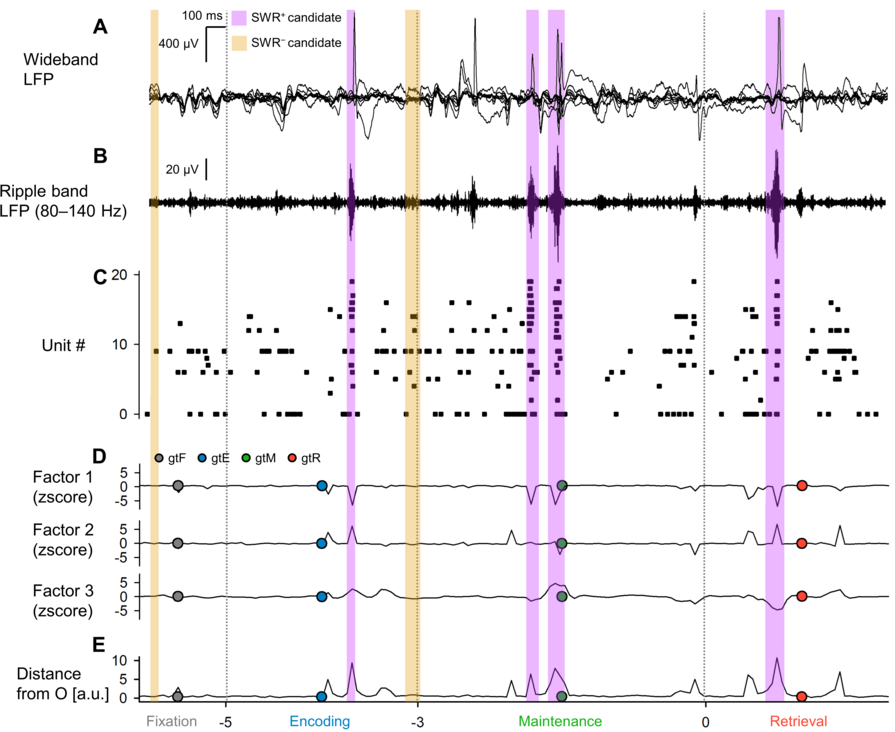
\includegraphics[width=1\textwidth]{./src/figures/.png/Figure_ID_01.png}
        	\caption{\textbf{
Local Field Potentials, Multiunit Activity, and Neural Trajectories in the Hippocampus during a Modified Sternberg Task
}
\smallskip
\\
\textbf{\textit{A.}} Presented are representative wideband LFP signals for an intracranial EEG recording from the left hippocampal head, obtained while the subject performed a modified Sternberg working memory task. The task comprises stages of fixation (1s, \textit{gray}), encoding (2s, \textit{blue}), maintenance (3s, \textit{green}), and retrieval (2s, \textit{red}). \textbf{\textit{B.}} Depicted are the associated ripple band LFP traces. Pay attention to the \textit{purple} and \textit{yellow} rectangles, which represent the timings for SWR$^+$ candidates and SWR$^-$ candidates, respectively (the latter serve as control events for SWR$^+$). \textbf{\textit{C.}} A raster plot demonstrates multi-unit spikes obtained from the LFP traces, sorted using a spike algorithm \cite{niediek_reliable_2016}. \textbf{\textit{D.}} The neural trajectories (NTs) calculated by GPFA\cite{yu_gaussian-process_2009} based on spike counts per unit with 50-ms bins are displayed; the geometric median of each phase is marked by dot circles. \textbf{\textit{E.}} The distance of the NT from the origin point $O$ is shown.
}
% width=1\textwidth
        	\label{fig:01}
        \end{figure*}
        \clearpage
        \begin{figure*}[ht]
            \pdfbookmark[2]{ID 02}{figure_id_02}
        	\centering
            \includegraphics[width=]{./src/figures/.png/Figure_ID_02.png}
        	\caption{\textbf{
State-Dependent Neural Trajectories of Hippocampal Neurons
}
\smallskip
\\
\textbf{\textit{A.}} Neural trajectories (NTs) are represented as a point cloud within the first three-dimensional factors derived from Gaussian Process Factor Analysis (GPFA) \cite{yu_gaussian-process_2009}. The smaller dots represent 50-ms NT bins, while the larger dots with black edges denote the geometric medians for each phase of the Sternberg working memory task. These phases include fixation ($\mathrm{\lVert g_{F} \rVert}$, gray), encoding ($\mathrm{\lVert g_{E} \rVert}$, blue), maintenance ($\mathrm{\lVert g_{M} \rVert}$, green), and retrieval ($\mathrm{\lVert g_{R} \rVert}$, red). \textbf{\textit{B.}} The figure shows the log-likelihood of GPFA models against the number of dimensions used to embed multi-unit spikes found in the medial temporal lobe (MTL) regions. Specifically, the elbow method identified three as the optimal dimension. \textbf{\textit{C.}} This panel depicts the distance of the NTs from the origin ($O$) for the hippocampus (Hipp.), entorhinal cortex (EC), and amygdala (Amy.), plotted against the elapsed time since probe onset. \textbf{\textit{D.}} Here, the NT distance from $O$ within the MTL regions is displayed. The greatest distance is in the hippocampus, followed by the EC and the Amygdala. \textbf{\textit{E.}} The box plot shows the inter-phase NT distances within the MTL regions.
}
        	\label{fig:02}
        \end{figure*}
        \clearpage
        \begin{figure*}[ht]
            \pdfbookmark[2]{ID 03}{figure_id_03}
        	\centering
            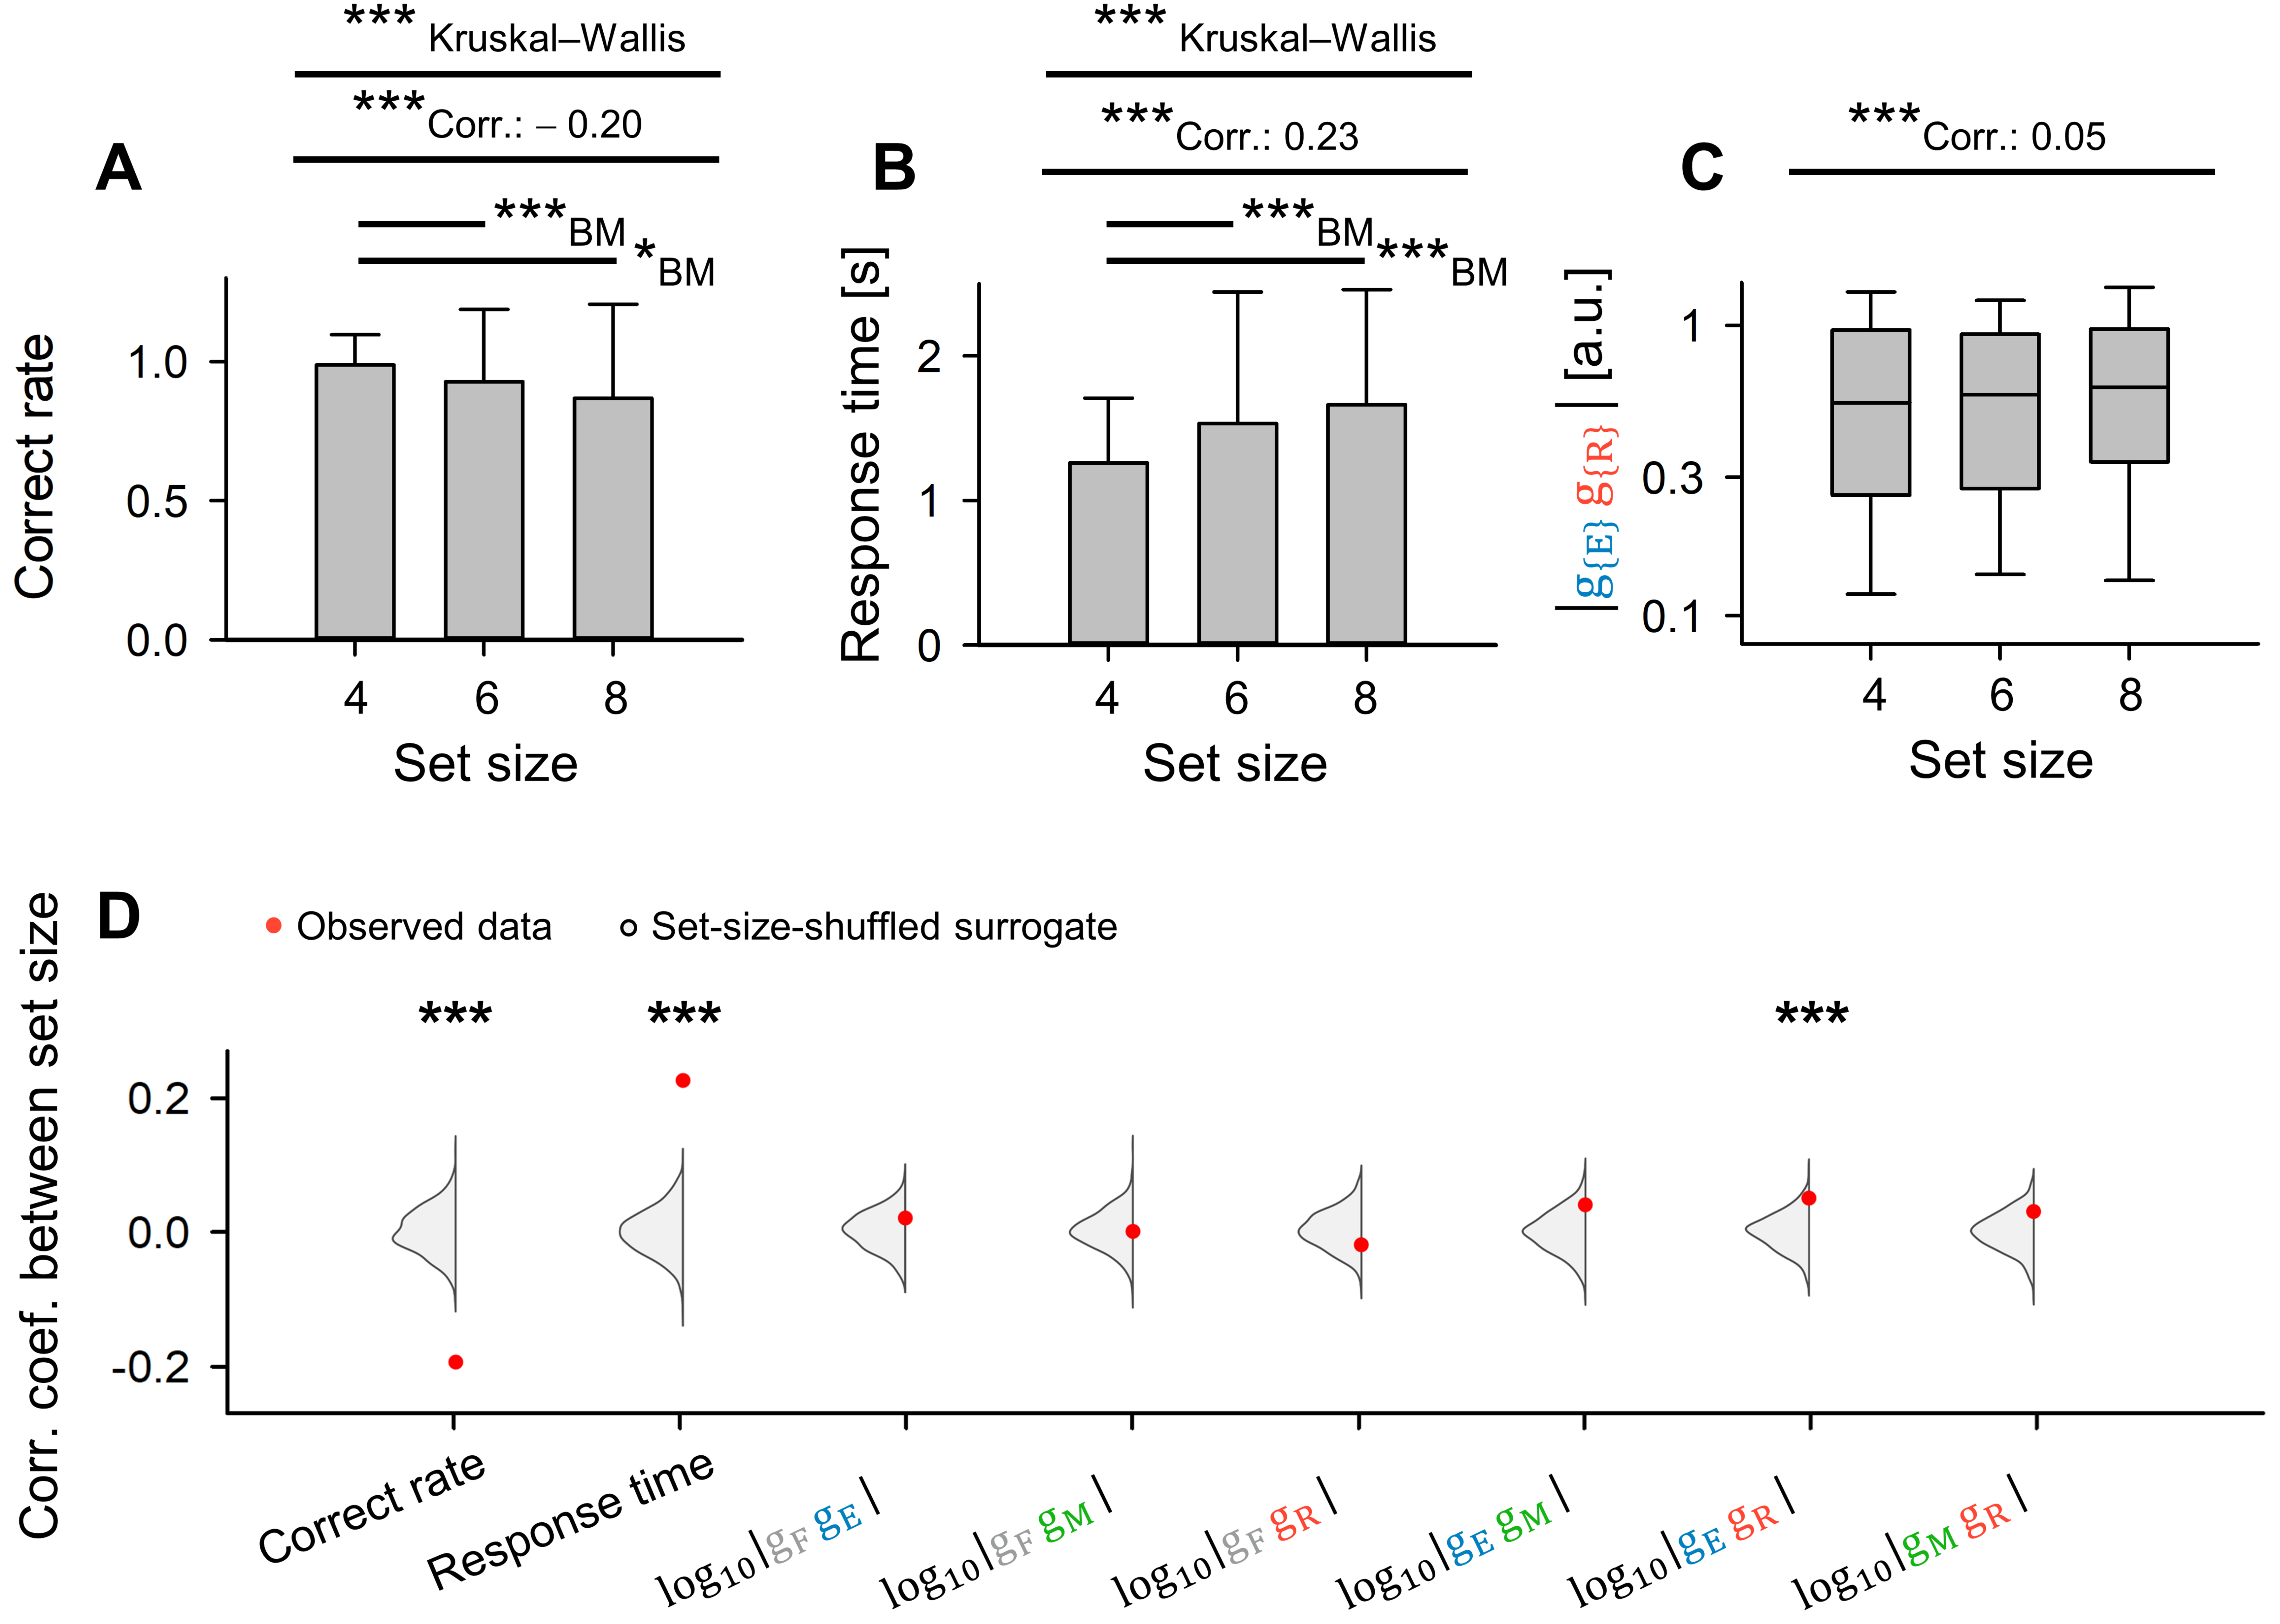
\includegraphics[width=1\textwidth]{./src/figures/.png/Figure_ID_03.png}
        	\caption{\textbf{
Positive Correlation Between Memory Load and Neural Trajectory Distance in the Hippocampus during Encoding and Retrieval Phases
}
\smallskip
\\
\textbf{\textit{A.}} Relationship between set size (number of encoded letters) and accuracy in the working memory task (coefficient = $-0.20$, ***\textit{p} $<$ 0.001). \textbf{\textit{B.}} Correlation between set size and response time (coefficient = 0.23, ***\textit{p} $<$ 0.001). \textbf{\textit{C.}} Correlation of set size with the inter-phase distances between encoding and retrieval phases ($\lVert \mathrm{g_{E}g_{R}} \rVert$) (correlation coefficient = 0.05, ***\textit{p} $<$ 0.001). \textbf{\textit{D.}} Experimental correlations between set size and the following parameters: accuracy, response time, $\log_{10}{\lVert \mathrm{g_{F}g_{E}} \rVert}$, $\log_{10}{\lVert \mathrm{g_{F}g_{M}} \rVert}$, $\log_{10}{\lVert \mathrm{g_{F}g_{R}} \rVert}$, $\log_{10}{\lVert \mathrm{g_{E}g_{M}} \rVert}$, $\log_{10}{\lVert \mathrm{g_{E}g_{R}} \rVert}$, and $\log_{10}{\lVert \mathrm{g_{M}g_{R}} \rVert}$ represented by \textit{red} dots. The kernel density plots (\textit{gray}) illustrate the corresponding shuffled surrogate with set size (\textit{n} = 1,000) (***\textit{p}s $<$ 0.001).
}
% width=1\textwidth
        	\label{fig:03}
        \end{figure*}
        \clearpage
        \begin{figure*}[ht]
            \pdfbookmark[2]{ID 04}{figure_id_04}
        	\centering
            \includegraphics[width=1\textwidth]{./src/figures/.png/Figure_ID_04.png}
        	\caption{\textbf{Detection of Sharp Wave Ripples in Presumed CA1 Regions}\\
\textbf{\textit{A.}} A two-dimensional UMAP \cite{mcinnes_umap_2018} projection illustrates multi-unit spikes during positive sharp wave ripples (SWR$^+$) candidates (\textit{purple}) and negative sharp wave ripples (SWR$^-$) candidates (\textit{yellow}). \textbf{\textit{B.}} A cumulative density plot shows silhouette scores, which reflect the quality of UMAP clustering (refer to Table~\ref{tab:02}). Presumed CA1 regions are identified by silhouette scores greater than 0.60 (equivalent to the 75th percentile). Hits and misses recorded from these regions are classified as SWR$^+$ and SWR$^-$ accordingly (\textit{n}s = 1,170). \textbf{\textit{C.}} Consistent distributions of durations for SWR$^+$ (\textit{purple}) and SWR$^-$ (\textit{yellow}) are demonstrated, as defined by the median interquartile range (IQR) of 93.0 [65.4] ms. \textbf{\textit{D.}} The occurrence of SWR$^+$ (\textit{purple}) and SWR$^-$ (\textit{yellow}), in relation to the probe's timing, is depicted as a mean \textpm 95\% confidence interval. Please note that the intervals may not be visibly discernible due to their confined ranges, despite a significant surge in SWR incidence during the initial 400 ms of the retrieval phase (0.421 [Hz], *\textit{p} $<$ 0.05, bootstrap test). \textbf{\textit{E.}} The distributions of ripple band peak amplitudes for SWR$^-$ (\textit{yellow}; 2.37 [0.33] SD of baseline, median [IQR]) and SWR$^+$ (\textit{purple}; 3.05 [0.85] SD of baseline, median [IQR]) are depicted (***\textit{p} $<$ 0.001, the Brunner--Munzel test).} % width=1\textwidth
        	\label{fig:04}
        \end{figure*}
        \clearpage
        \begin{figure*}[ht]
            \pdfbookmark[2]{ID 05}{figure_id_05}
        	\centering
            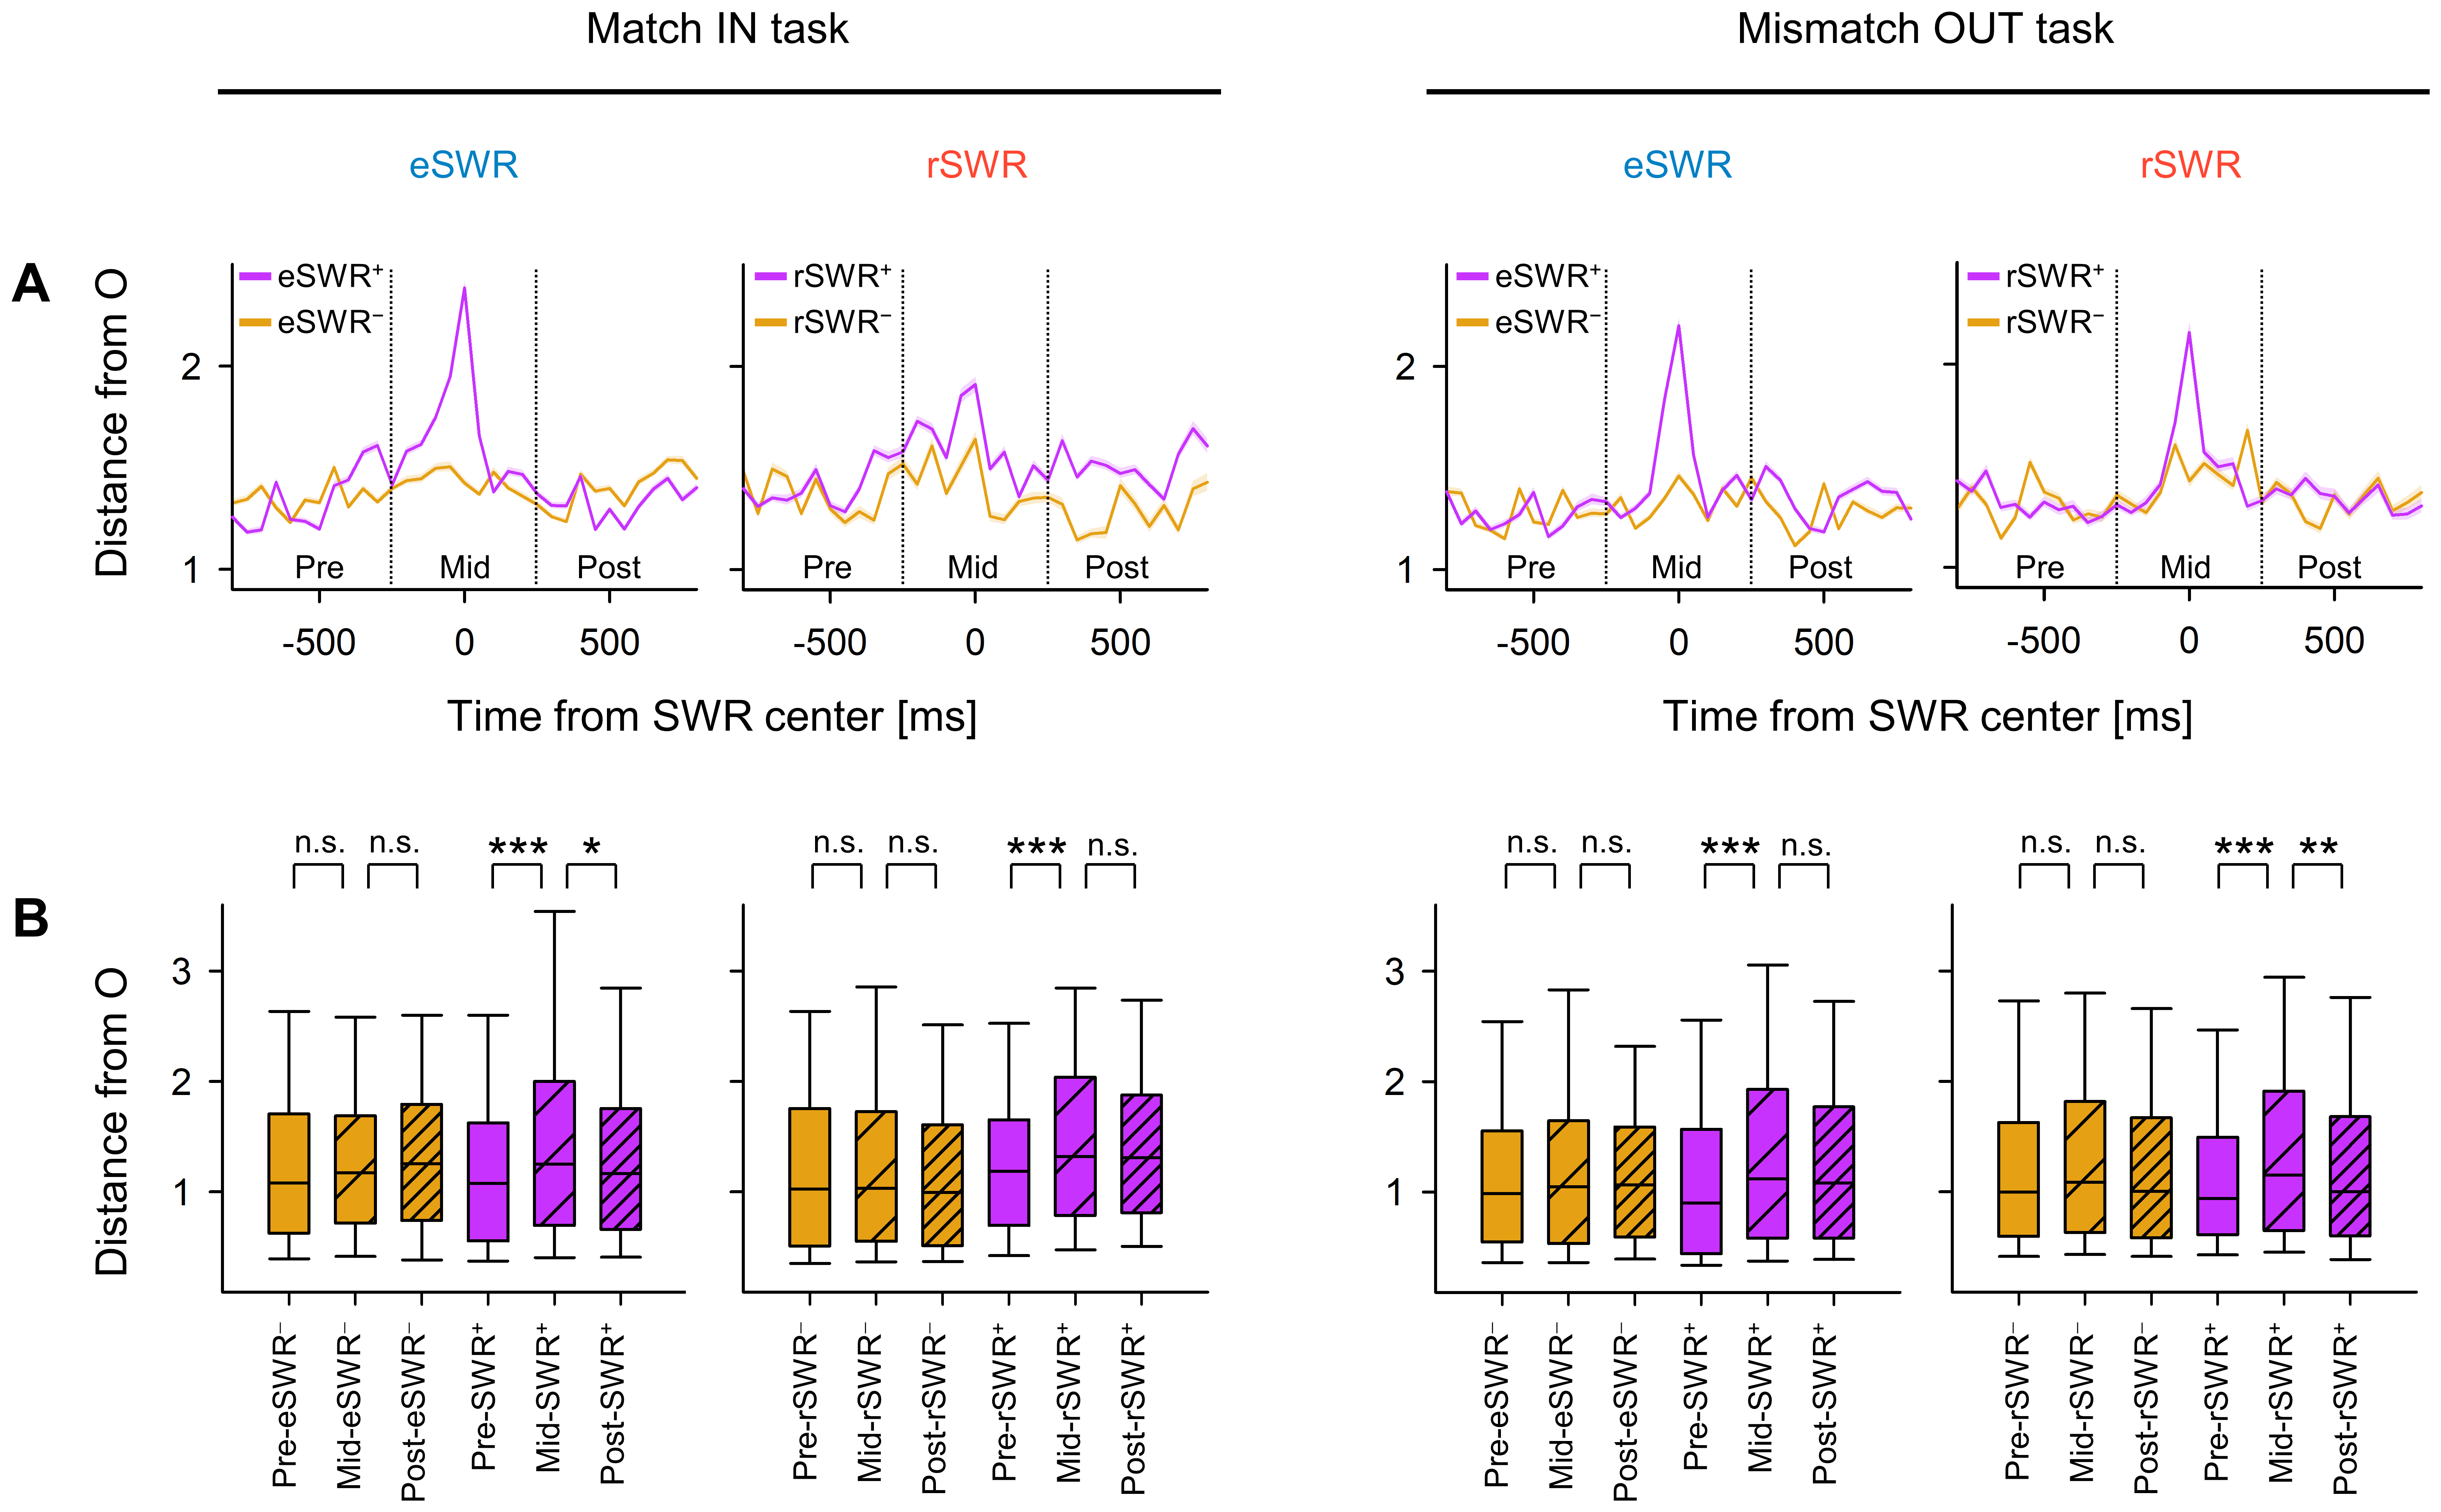
\includegraphics[width=1\textwidth]{./src/figures/.png/Figure_ID_05.png}
        	\caption{\textbf{Transient Change in Neural Trajectory during Sharp-Wave Ripple Events}
\smallskip
\\
\textbf{\textit{A.}} Distance from origin ($O$) of the peri-sharp-wave-ripple neural trajectory (mean \textpm 95\% confidence interval). Intervals may be inconspicuous due to their minimal ranges. \textbf{\textit{B.}} Distance from the origin ($O$) during the pre-, mid-, and post-sharp-wave ripple periods is demonstrated (*\textit{p} $<$ 0.05, **\textit{p} $<$ 0.01, ***\textit{p} $<$ 0.001; Brunner--Munzel test applied). Abbreviations: SWR, sharp-wave ripple event; eSWR, sharp-wave ripple during the encoding phase; rSWR, sharp-wave ripple within the retrieval phase; SWR$^+$, positive sharp-wave ripple event; SWR$^-$, control events for SWR$^+$; pre-, mid-, or post-SWR refer to the time intervals from $-800$ to $-250$ ms, from $-250$ to $+250$ ms, or from $+250$ to $+800$ ms, respectively, all relative to the center of the sharp-wave ripple event.}
% width=1\textwidth
        	\label{fig:05}
        \end{figure*}
        \clearpage
        \begin{figure*}[ht]
            \pdfbookmark[2]{ID 06}{figure_id_06}
        	\centering
            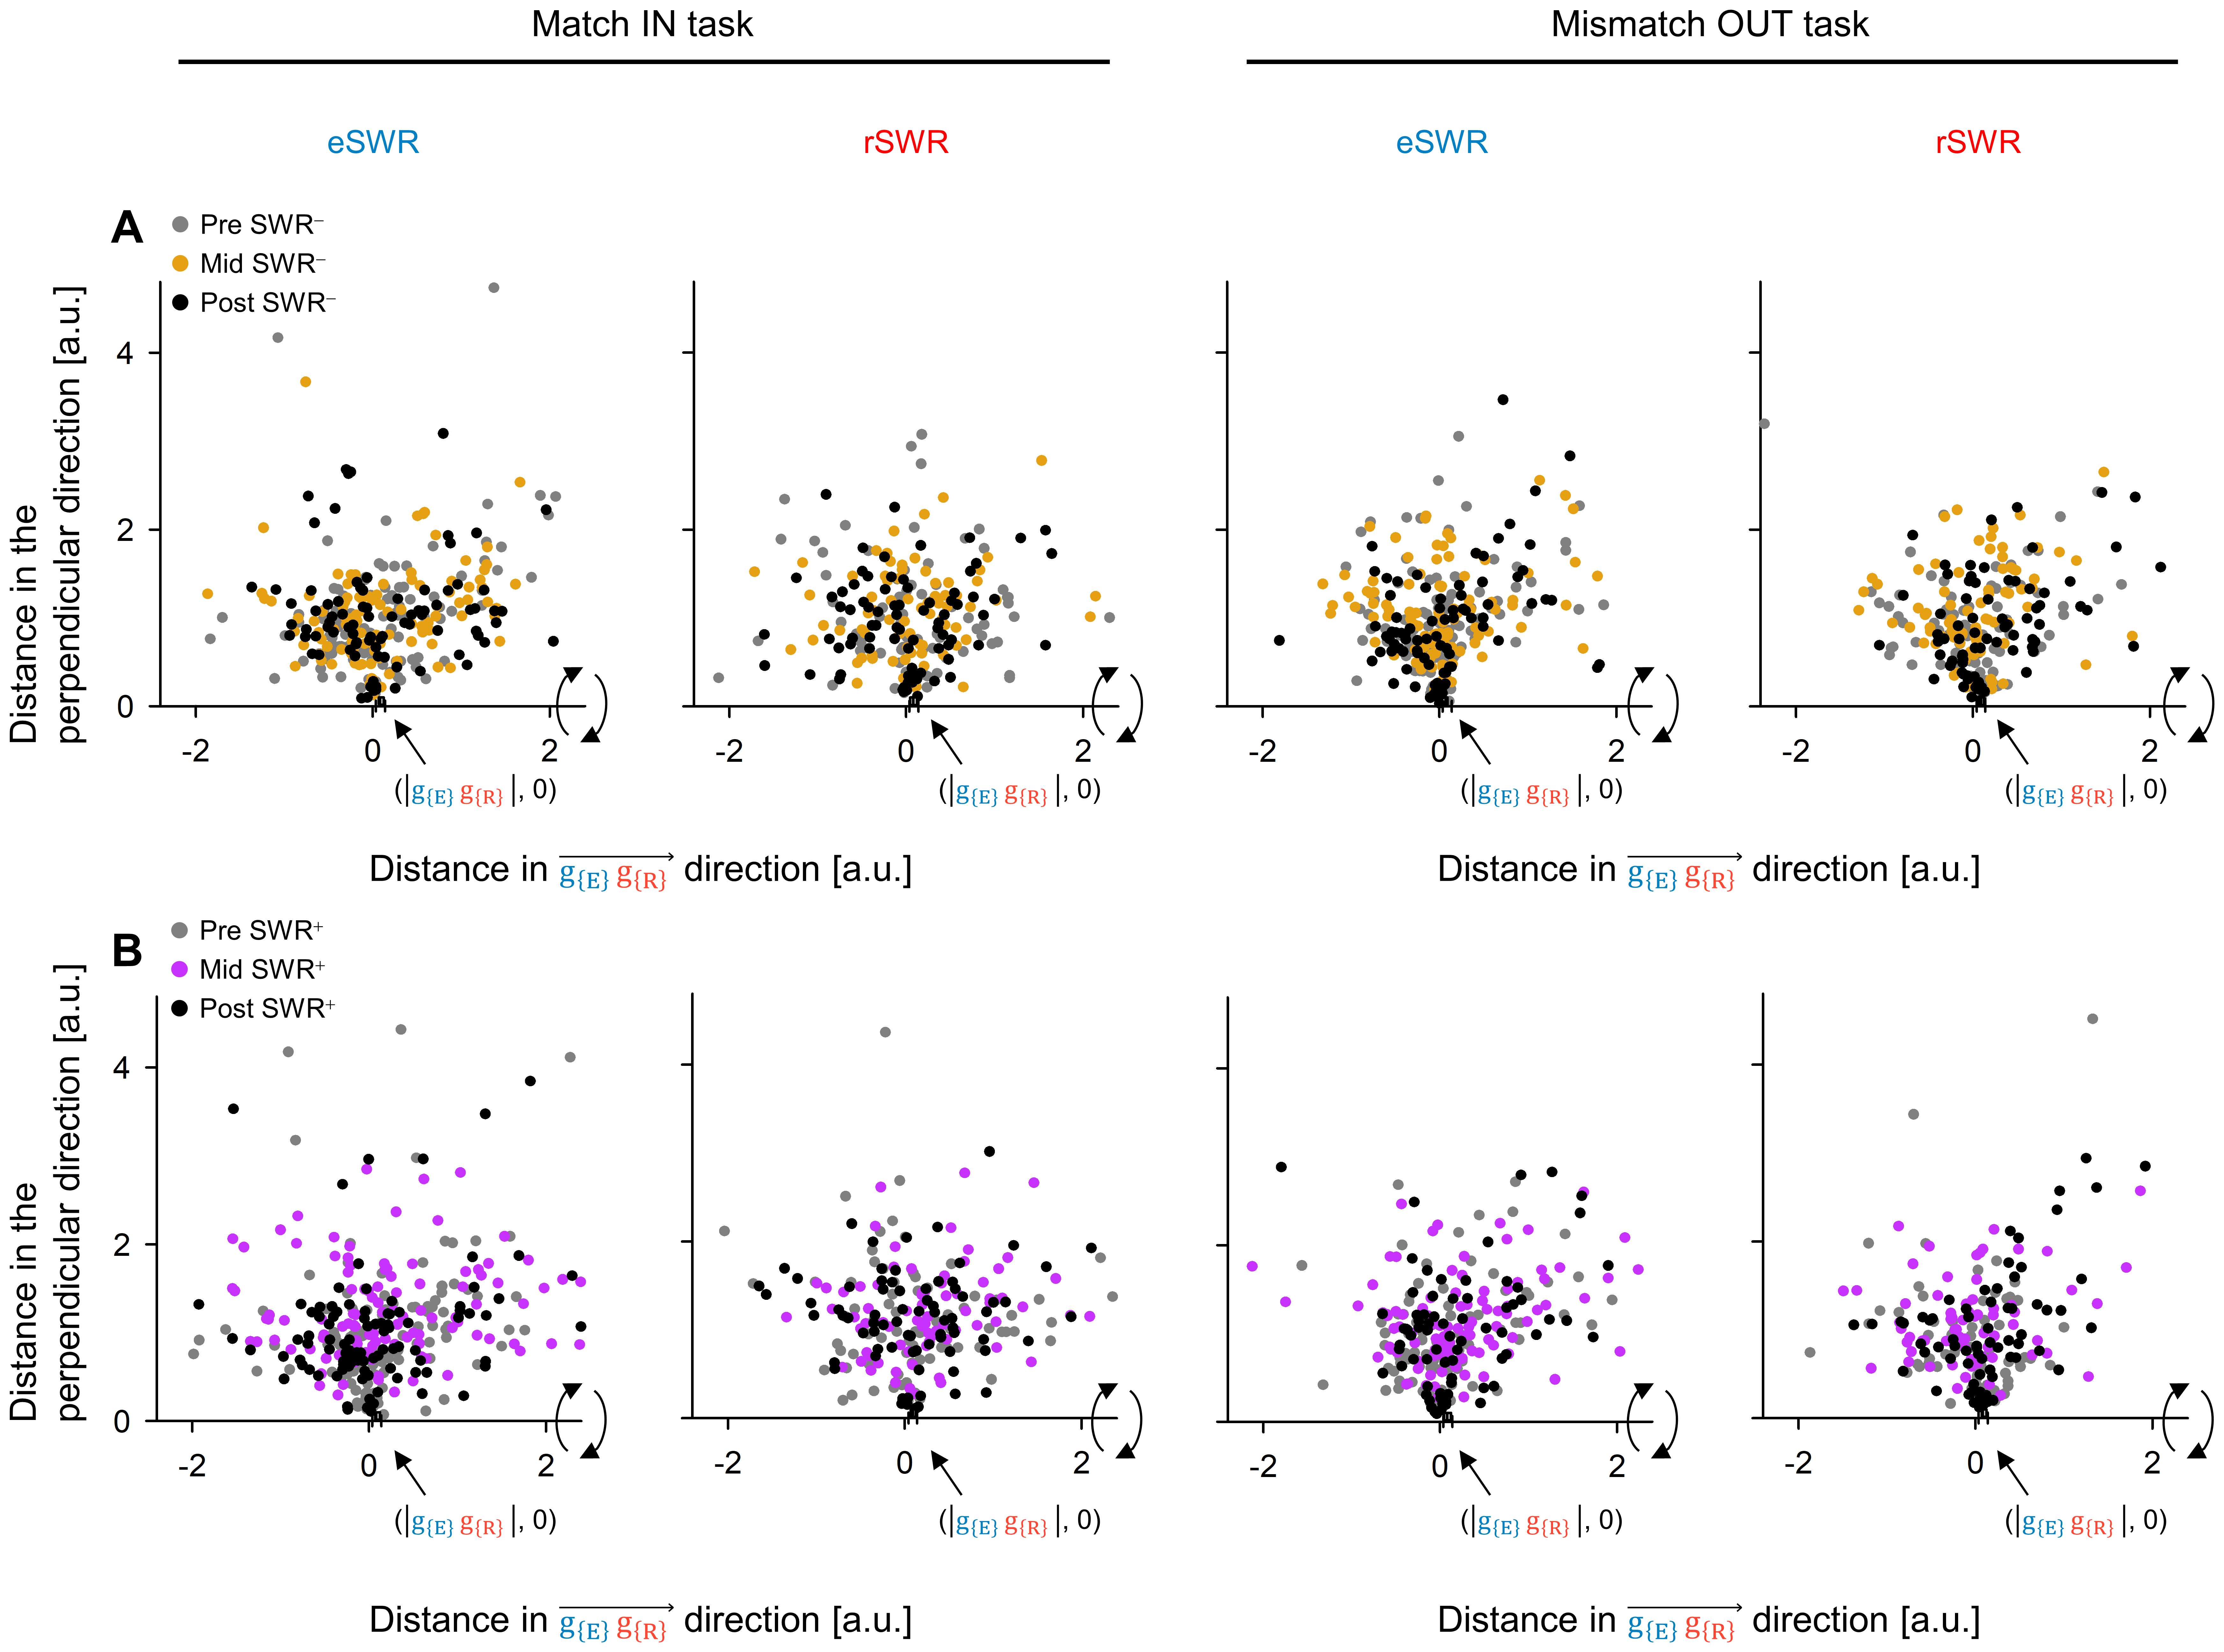
\includegraphics[width=]{./src/figures/.png/Figure_ID_06.png}
        	\caption{\textbf{Visualization of Neural Trajectories during Sharp-Wave Ripple Events in Two-Dimensional Space}
\smallskip
\\
The panels portray hippocampal neural trajectories (NTs) during sharp-wave ripple (SWR) events, projected onto two-dimensional spaces. \textbf{\textit{A.}} Displays the hippocampal NTs as point clouds during pre-SWR$^-$ (in gray), mid-SWR$^-$ (in yellow), and post-SWR$^-$ (in black). \textbf{\textit{B.}} Presents the comparable depiction for SWR$^+$ instead of SWR$^-$. The projection was undertaken as follows: Firstly, a linear transformation set $\mathrm{g_{E}}$ at the origin point $O$ (0,0), and $\mathrm{g_{R}}$ at ($\lVert \mathrm{g_{E}g_{R}} \rVert$, 0). Subsequently, the point cloud was rotated around the $\mathrm{g_{E}g_{R}}$ axis (akin to the x-axis), adjusting it to two-dimensional spaces. As such, in these two-dimensional spaces, the distances from point $O$ and the angles for the $\mathrm{g_{E}g_{R}}$ axis are preserved identically as in the original three-dimensional spaces generated by Gaussian Process Factor Analysis (GPFA). Abbreviations: SWR denotes sharp-wave ripple events; encoding sharp-wave ripple (eSWR) refers to SWR during the encoding phase; retrieval sharp-wave ripple (rSWR) indicates SWR during the retrieval phase; SWR$^+$ characterizes a SWR event; SWR$^-$ designates control events for SWR$^+$; pre-SWR, mid-SWR, or post-SWR define the time intervals from $-800$ to $-250$ ms, from $-250$ to $+250$ ms, or from $+250$ to $+800$ ms from the center of SWR, respectively.
}
        	\label{fig:06}
        \end{figure*}
        \clearpage
        \begin{figure*}[ht]
            \pdfbookmark[2]{ID 07}{figure_id_07}
        	\centering
            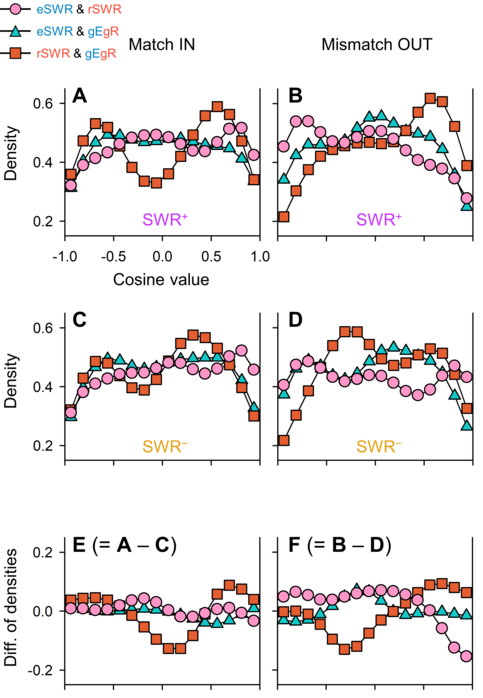
\includegraphics[width=0.5\textwidth]{./src/figures/.png/Figure_ID_07.png}
        	\caption{\textbf{
Direction of Neural Trajectory during SWR Based on Encoding and Retrieval States
}
\smallskip
\\
\textbf{\textit{A--B}} The kernel density estimation distributions of $\protect\overrightarrow{{\mathrm{eSWR^+}}}$ $\cdot$ $\protect\overrightarrow{{\mathrm{rSWR^+}}}$ (\textit{pink circles}), $\protect\overrightarrow{{\mathrm{eSWR^+}}}$ $\cdot$ $\protect\overrightarrow{{\mathrm{g_{E}g_{R}}}}$ (\textit{blue triangles}), and $\protect\overrightarrow{{\mathrm{rSWR^+}}}$ $\cdot$ $\protect\overrightarrow{{\mathrm{g_{E}g_{R}}}}$ (\textit{red rectangles}) in Match In (\textit{A}) and Mismatch OUT tasks (\textit{B}). \textbf{\textit{C--D}} The corresponding distributions of $\mathrm{SWR^-}$ to those of $\mathrm{SWR^+}$ in \textit{A} and \textit{B}. \textbf{\textit{E--F}} The differential distributions of $\mathrm{SWR^+}$ and $\mathrm{SWR^-}$, demonstrating SWR components (\textit{E} = \textit{C} - \textit{A}, \textit{F} = \textit{D} - \textit{B}). Biphasic distributions of $\protect\overrightarrow{{\mathrm{rSWR^-}}}$ $\cdot$ $\protect\overrightarrow{{\mathrm{g_{E}g_{R}}}}$ signal fluctuations between the encoding and retrieval states during the Sternberg task. A contrasting directionality between $\protect\overrightarrow{{\mathrm{eSWR^+}}}$ and $\protect\overrightarrow{{\mathrm{rSWR^+}}}$ is noticeable (pink circles) not in the Match IN task (\textbf{\textit{E}}), but in the Mismatch OUT task (\textbf{\textit{F}}). Lastly, transitions from the retrieval to encoding states are apparent in the SWR components in both Match IN and Mismatch OUT tasks (\textit{red rectangles} in \textit{E--F}).
}
% width=0.5\textwidth
        	\label{fig:07}
        \end{figure*}

%%%%%%%%%%%%%%%%%%%%%%%%%%%%%%%%%%%%%%%%%%%%%%%%%%%%%%%%%%%%%%%%%%%%%%%%%%%%%%%%
%% END
%%%%%%%%%%%%%%%%%%%%%%%%%%%%%%%%%%%%%%%%%%%%%%%%%%%%%%%%%%%%%%%%%%%%%%%%%%%%%%%%

\end{document}
